\documentclass{beamer}
\usepackage{preamble}


% TITLE PAGE INFORMATION
\title{MyBeamerTemplate}
%\subtitle{}
\author{Lorenzo Squadrani}
%\institute{University of Bonn}
\date{\today}



\begin{document}

    \begin{frame}
    \titlepage    
    \end{frame}

    \begin{frame}{Well aligned columns}
        \begin{columns}
            \begin{column}[T]{0.49\textwidth}
                \centering \textbf{Column 1}

                \begin{minipage}[t][3cm][t]{\textwidth}
                \begin{equation*}
                    E = m c^2
                \end{equation*}
                \end{minipage}
                \vspace{0.1cm}
                
                Some comment 1
            \end{column}
            \begin{column}[T]{0.49\textwidth}
                \centering \textbf{Column 2}

                \begin{minipage}[t][3cm][t]{\textwidth}
                \begin{equation*}
                    F = ma
                \end{equation*}
                \begin{equation*}
                    \ddot x = - x
                \end{equation*}
                \end{minipage}
                \vspace{0.1cm}
                
                Some comment 2
            \end{column}
        \end{columns}
    \end{frame}

    \begin{frame}{Drawing on pictures}
        \begin{figure}
            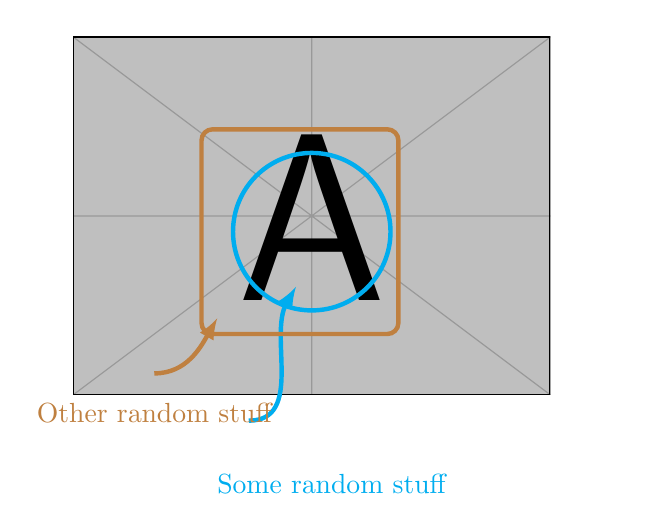
\begin{tikzpicture}
                \node at (0, 0) {\includegraphics[width=0.5\textwidth]{example-image-a}};
                
                \draw[ultra thick, cyan] (0,-0.2) circle (1cm);
                \draw [-latex, ultra thick, cyan] (-0.8,-2.6) to[out=0, in=-120] (-0.2, -0.9);
                \node at (1.3, -3.4) [text width=5cm]{\color{cyan}Some random stuff};

                \node at (-2, -2.5){\color{brown} Other random stuff};
                \draw[brown,ultra thick,rounded corners] (-1.4,-1.5) rectangle (1.1, 1.1);
                \draw [-latex, ultra thick, brown] (-2, -2) to[out=0, in=-120] (-1.2, -1.3);
            \end{tikzpicture}
        \end{figure}
    \end{frame}

    \begin{frame}{Rounded images with bullet lists}
    \begin{columns}
        \begin{column}{0.49\textwidth}
            \begin{itemize}
                \item item 1
                \item item 2
                \item item 3
            \end{itemize}
            \begin{figure}
                \centering
                \cutpic{0.3cm}{\textwidth}{example-image-a}
            \end{figure}
        \end{column}
        \begin{column}{0.49\textwidth}
            \begin{figure}
                \centering
                \cutpic{0.3cm}{\textwidth}{example-image-b}
            \end{figure}
            \vspace{0.5cm}
            \begin{itemize}
                \item item 1
                \item item 2
            \end{itemize}
            \vspace{1cm}
        \end{column}
    \end{columns}
    \end{frame}

    
    \begin{frame}{A collage of pictures}

    \begin{figure}
        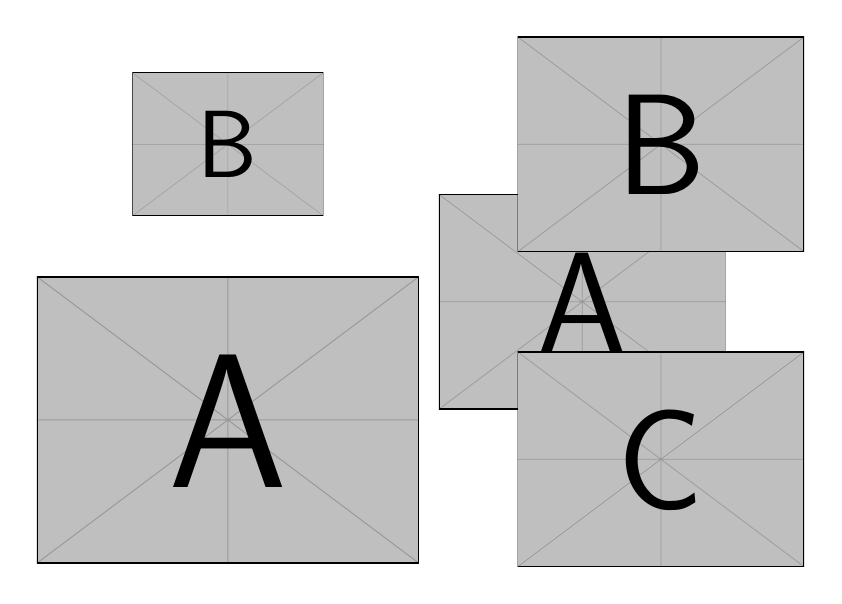
\begin{tikzpicture}
            \node at (2,0) {\includegraphics[width=0.3\textwidth]{example-image-a}};
            \node at (-2.5, 2) {\includegraphics[width=0.2\textwidth]{example-image-b}};
            \node at (3, -2) {\includegraphics[width=0.3\textwidth]{example-image-c}};
            \node at (-2.5, -1.5) {\includegraphics[width=0.4\textwidth]{example-image-a}};
            \node at (3, 2) {\includegraphics[width=0.3\textwidth]{example-image-b}};
        \end{tikzpicture}
    \end{figure}
    \end{frame}

    
    \begin{frame}{Custom fillable forms}
    
        \begin{Form}
           Name: \TextField[width=0.5\textwidth]{}{}
        \end{Form}
    
    \end{frame}
    
\end{document}
